\chapter{Beispiele}
\section{Tools}
In den nachfolgenden Beispielen kam das HeuristicLab als Tool zur Anwendung,
welches bei der Berechnung komplexer heuristischer Daten Anwendung findet.
Diese Software wurde von der FH Hagenberg entwickelt und steht kostenfrei zur Verfügung. Bei den Tests wurde diese Software zum Berechnen von Klassifikationen und Clustern genutzt um die verschiedenen Algorithmen zu vergleichen. Die Testdaten liegen in Format \(.csv\) vor und sind durch einen \(;\) getrennt.
\section{Klassifikation}
\subsection{Einführung}
Nachfolgend wird die Klassifikation anhand mehrerer Datensätze gezeigt, dabei wird der \textit{Nearest Neigbour} Algorithmus verwendet. Alle Datensätze wurden vom \textit{UCI Repository} herangezogen und beinhalten jeweils die notwendigen Daten wie der Klassenzuordnung. Es werden immer die Datensätze anhand der \textit{Confusion Matrix} bewertet, welche angibt wie gut der Klassifikator ist. \cite{uci}
\subsection{Iris Datensatz}
Dieser Datensatz ist der bekannteste auf dem Gebiet von Data Minig und der Klassifikation und wird zum Testen von Erkennungsmerkmalen von zusammengehörigen Formen verwendet. Daher ist dieser Datensatz auch zum Testen für die Klassifikation geeignet. \cite{uci}
\subsubsection{Eingabedaten}
\begin{itemize}
	\item Klassen: 3
	\item Datengröße: 150
\end{itemize}
\subsubsection{Parameter}
\begin{itemize}
	\item Train: 33\% Test: 67\%
	\item K: 3 
\end{itemize}
\subsubsection{Ergebnis}
\begin{figure}[H]
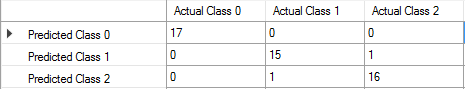
\includegraphics[width=\textwidth]{Iris_Test_CM.png}
\caption{Confusion Matrix}
\label{}
\end{figure}

Aus der Klasseneinteilung lässt sich die Genauigkeit bestimmen, welche hier 96\% beträgt. Der \textit{gini-index} daher ist 0,98 .

\subsection{Wisconsin Diagnostic Breast Cancer Datensatz}
Die Werte stammen aus einem digitalen Bild und beschreiben die Beschaffenheit der einzeln Zellen im Gewebe welche auf dem Bild zu sehen sind. \cite{uci}
\subsubsection{Eingabedaten}
\begin{itemize}
	\item Klassen: 2
	\item Datengröße: 569
\end{itemize}
\subsubsection{Parameter}
\begin{itemize}
	\item Train: 33\% Test: 67\%
	\item K: 3 
\end{itemize}
\subsubsection{Ergebnis}
\begin{figure}[H]
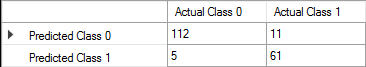
\includegraphics[width=\textwidth]{Cancer_Test_CM.png}
\caption{Confusion Matrix}
\end{figure}

Aus der Klasseneinteilung lässt sich die Genauigkeit bestimmen, welche hier 91.5\% beträgt. Der \textit{gini-index} daher ist 0,86 .

\subsection{Parkinsons Datensatz}
Der Datensatz stammt von 31 Personen, bei denen die Stimmen gemessenen worden sind, diesbezüglich hatten 23 die Krankheit Parkinson. \cite{uci}
\subsubsection{Eingabedaten}
\begin{itemize}
	\item Klassen: 2
	\item Datengröße: 195
\end{itemize}
\subsubsection{Parameter}
\begin{itemize}
	\item Train: 33\% Test: 67\%

	\item K: 7
\end{itemize}
\subsubsection{Ergebnis}
\begin{figure}[H]
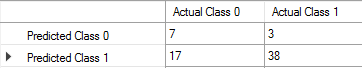
\includegraphics[width=\textwidth]{Parkinsons_Test_CM.png}
\caption{Confusion Matrix}
\end{figure}

Aus der Klasseneinteilung lässt sich die Genauigkeit bestimmen, welche hier 69.2\% beträgt. Der \textit{gini-index} ist daher 0,81.
\subsection{Fazit}
Aus den Ergebnissen kann ableitet werden, dass es bei der Klassifikation wichtig ist, das richtige Verhältnis zwischen Trainings- und Testdaten zu finden. Dies ist stark ausschlaggebend für die Qualität der Ergebnisse. Weiters ist auch zu beachten, dass das Verhältnis zwischen Datenreihen und Klassen entspricht, da sonst es zu Misklassifikationen kommen kann und dadurch zu einer Verschlechterung der Güte. Derzeitiger Stand ist, dass es keine wirkliche Regel für das Verhältnis zwischen Klassen und Anzahl der Daten gibt. Trotzdem sollte von einem relativ ausgeglichen Verhältnis ausgegangen werden.
\section{Clustering}
\subsection{Einführung}
Das Clustering wird anhand des \textit{k-means} Algorithmus gezeigt. Da ein Vergleich zwischen Clustering und Klassifikation erfolgen sollte, wurden herbei dieselben Datensätze verwendet. Der Unterschied zur Klassifikation ist, dass dabei die Klassendefinition weggelassen wird und stellt daher eine unüberwachte Klassifikation dar. Bei der Auswertung werden die Cluster gezeigt und die Zugehörigkeit gebildet. \cite{uci}
\subsection{Iris Datensatz}
\begin{itemize}
	\item Datengröße: 150
\end{itemize}
\subsubsection{Parameter}
\begin{itemize}
	\item K: 3 
	\item Wiederholungen: 0
\end{itemize}
\subsubsection{Ergebnis}
\begin{figure}[H]
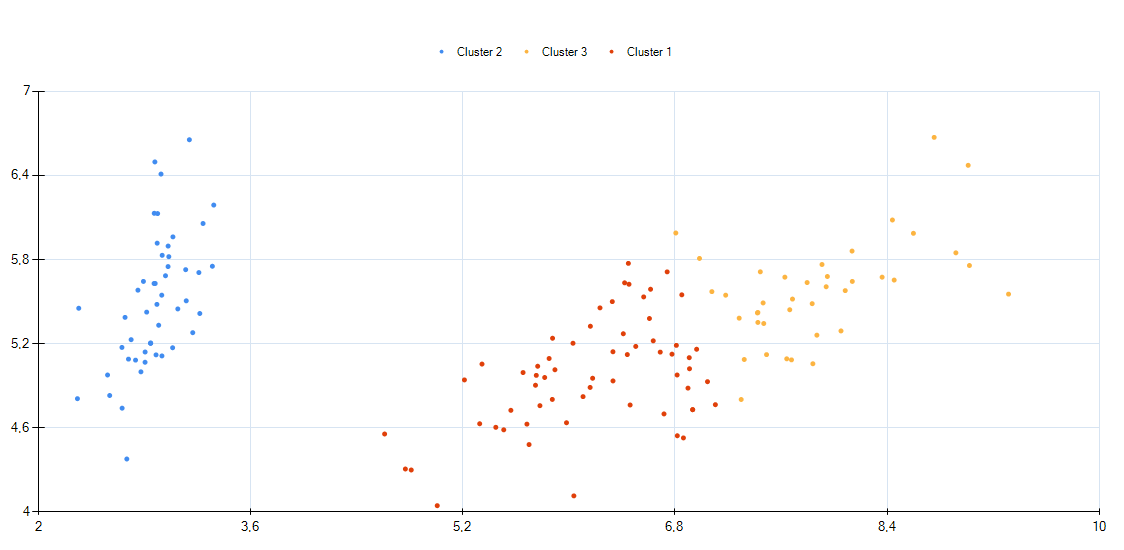
\includegraphics[width=\textwidth]{Iris_Test_CL.png}
\caption{Cluster}
\end{figure}

Wie zu erkennen ist gibt es wenige Ausreißer, da die Daten ursprünglich von einem Datensatz bezüglich Klassifikation stammen und bereits in Klassen dargestellt worden sind. 
\cite{uci}
\subsection{Wisconsin Diagnostic Breast Cancer Datensatz}
\begin{itemize}
	\item Datengröße: 569
\end{itemize}
\subsubsection{Parameter}
\begin{itemize}
	\item K: 3 
	\item Wiederholungen: 0
\end{itemize}
\subsubsection{Ergebnis}
\begin{figure}[H]
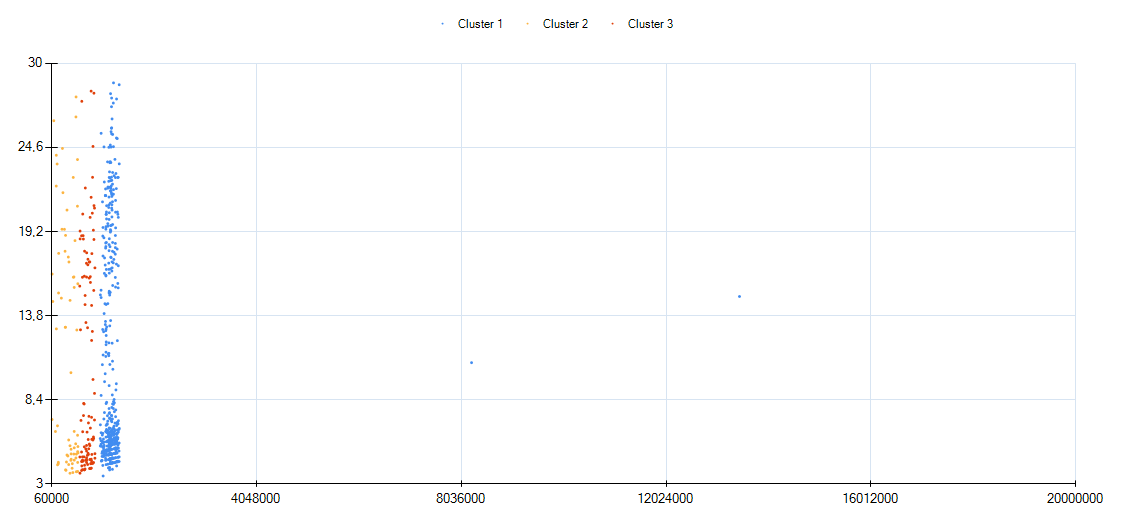
\includegraphics[width=\textwidth]{Cancer_Test_CL.png}
\caption{Cluster}
\end{figure}
Bei diesen Datensatz ist zu erkennen, dass es Ausreißer gibt,  diese werden trotzdem wegen der \textit{Ähnlichkeit} einiger Merkmale einem Cluster zugeordnet.
\cite{uci}
\subsection{Parkinsons Datensatz}
\begin{itemize}
	\item Datengröße: 195
\end{itemize}
\subsubsection{Parameter}
\begin{itemize}
	\item K: 2 
	\item Wiederholungen: 0
\end{itemize}
\subsubsection{Ergebnis}
\begin{figure}[H]
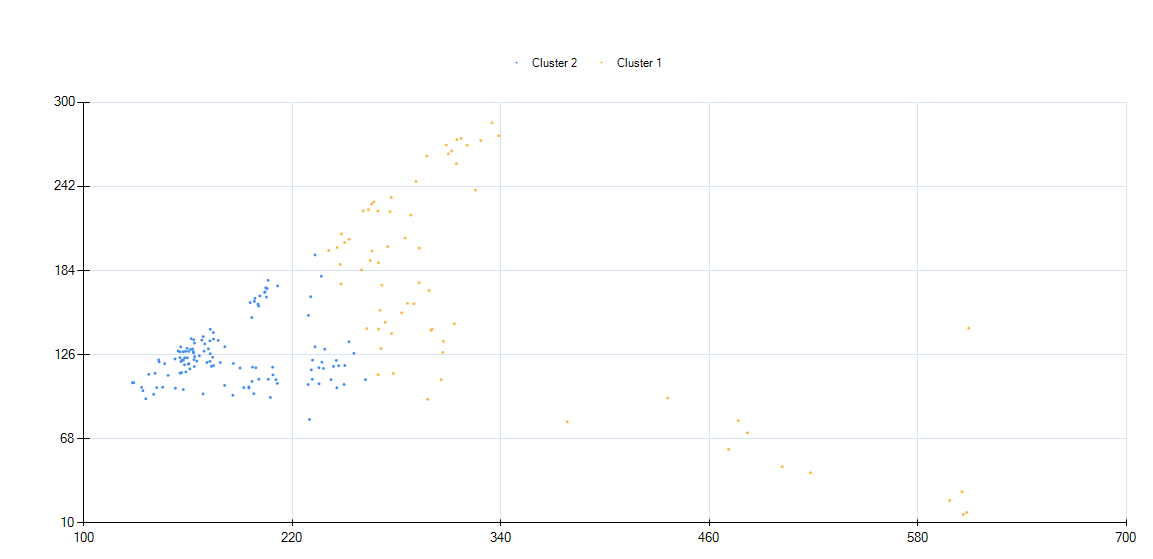
\includegraphics[width=\textwidth]{Parkinsons_Test_CL.png}
\caption{Cluster}
\end{figure}
Durch die Wahl von von zwei Clustern kann eine gute Klassifikation dargestellt werden, da die zwei vorgegeben Klassen relativ exakt dargestellt werden können 

\cite{uci}
\subsection{Fazit} 
Beim Clustering ist klar zu erkennen dass es Gemeinsamkeiten mit der Klassifikation gibt, da die meisten Clustereinteilungen die wahren Klassen voraussagen. Daher ist das Clustering ebenso bedeutend wie die Klassifikation. Beim Clustering kommt es auf die  vorgegebene Clusteranzahl an um gute Ergebnisse zu liefern.